\documentclass[10pt]{article}
\usepackage[T1]{fontenc}
\usepackage[utf8]{inputenc}
\usepackage[nottoc]{tocbibind}
\usepackage{graphicx}
\usepackage{subcaption}
\usepackage{indentfirst}
\usepackage[a4paper, margin=0.8in]{geometry}
\usepackage{hyperref}
\usepackage{float}
\usepackage[polish]{babel}
\usepackage[sorting=none]{biblatex}
\usepackage{csquotes}
\usepackage{amsfonts}
\usepackage{amsmath}
\usepackage{url}
\usepackage{algorithmicx}
\usepackage{algorithm}
\usepackage[noend]{algpseudocode}
\usepackage[dvipsnames]{xcolor}
\usepackage{tabularx}
\usepackage{subcaption}

\makeatletter
\newenvironment{breakablealgorithm}
  {% \begin{breakablealgorithm}
   \begin{center}
     \refstepcounter{algorithm}% New algorithm
     \hrule height.8pt depth0pt \kern2pt% \@fs@pre for \@fs@ruled
     \renewcommand{\caption}[2][\relax]{% Make a new \caption
       {\raggedright\textbf{\fname@algorithm~\thealgorithm} ##2\par}%
       \ifx\relax##1\relax % #1 is \relax
         \addcontentsline{loa}{algorithm}{\protect\numberline{\thealgorithm}##2}%
       \else % #1 is not \relax
         \addcontentsline{loa}{algorithm}{\protect\numberline{\thealgorithm}##1}%
       \fi
       \kern2pt\hrule\kern2pt
     }
  }{% \end{breakablealgorithm}
     \kern2pt\hrule\relax% \@fs@post for \@fs@ruled
   \end{center}
  }
\makeatother

\floatname{algorithm}{Algorytm}

\addbibresource{bibliography.bib}

\title{Mechanizm wymarcia w algorytmie CMA-ES \\
\large Dokumentacja wstępna}
\author{Szymon Stasiak \and Przemysław Woźniakowski}
\date{\today}

\begin{document}

\maketitle

\begin{abstract}
    Poniższy raport opisuje projekt, którego celem było przebadanie działania mechanizmu wymarcia populacji w algorytmie CMA-ES. W tym celu zaproponowany został sposób przeprowadzenia opartego na stagnacji mechanizmu wymarcia, wraz z dwoma jego wariantami. Zaproponowane warianty to wymieranie losowe, które polegało na odrzucaniu dowolnych punktów z populacji z pewnym prawdopodobieństwem, oraz wymieranie ukierunkowane, które wyłączało ze zbioru kandydatów do odrzucenia pewien odsetek najlepszych punktów. W ramach raportu opisane zostały eksperymenty, które miały na celu wyznaczyć optymalne parametry dla mechanizmu wymierania, czyli prawdopodobieństwo wymarcia oraz licznik stagnacji algorytmu, który decyduje kiedy dokonywane jest wymarcie. Dodatkowo opisane zostały eksperymenty na kilku przykładowych funkcjach  ze zbioru CEC 2022. Pokazały one, że mechanizm ukierunkowanego wymarcia poprawił uśrednioną skuteczność dla funkcji takich jak funkcja Schaffera i Rastrigina, nie dał jednak żadnych pozytywnych efektów jeśli chodzi o funkcję Levy'ego.
\end{abstract}

\tableofcontents

\newpage

\section{Opis problemu}

Tematem pracy jest połączenie dwóch konceptów stosowanych w algorytmach ewolucyjnych - algorytmu CMA-ES oraz mechanizmu wymarcia.

Nazwa algorytmu CMA-ES jest akronimem angielskiej nazwy Covariance Matrix Adaptation - Evolution Strategy. Na polski język można przetłumaczyć to jako strategie ewolucyjną bazującą na adaptacji macierzy kowariancji. Twórcami tego algorytmu są N. Hansen i A. Ostermaier, którzy w 2001 roku zamieścili jego opis w pracy \textit{Completely derandomized self-adaptation in evolution strategies} \cite{hansen2011}.

Algorytm CMA-ES skupia się przede wszystkim na sposobie generowania osobników w kolejnych pokoleniach (etapie selekcji). Otwiera to drogę do modyfikowania innych etapów. Jedną z takich modyfikacji jest prezentowane w tej pracy rozszerzenie o mechanizm wymarcia.

Sam w sobie mechanizm wymarcia w algorytmach ewolucyjnych jest konceptem znanym, jednak często uznawanym za nieznaczący. Niemniej jednak istnieją badania pokazujące korzystny wpływ tego konceptu na osiągane rezultaty. Jedną z takich prac jest powstały w 2021 roku artykuł autorstwa Gan Zhen Ye oraz Dae-Ki Kang \textit{Extended Evolutionary Algorithms with Stagnation-Based Extinction Protocol} \cite{ye2021}. Artykuł ten opisuje dwie implementacje opartego o stagnację mechanizmu wymarcia - wymarcie losowe oraz wymarcie ukierunkowane. Właśnie te dwie wersje zostały zaimplementowane i przeanalizowane w obrębie pracy. Głównym celem badania było zweryfikowanie, czy powszechna opinia o nieznaczącym wpływie na mechanizm wymarcia jest zasadna w przypadku CMA-ES, czy może jest to obiecujący kierunek rozwoju.

%Główną motywacją do powstania tego algorytmu była chęć lepszego dopasowania rozkładu osobników generowanych w kolejnych iteracjach do dynamiki funkcji celu. Zostało to osiągnięte poprzez modyfikację macierzy kowariancji używanej do generowania losowych punktów w fazie selekcji kolejnych pokoleń. Wartości w macierzy zostały uzależnione między innymi od wektorów odległości między kolejnymi wartościami oczekiwanymi rozkładu. W ten sposób jeżeli osobniki w kolejnych pokoleniach \textquote{przesuwają} się w stałym kierunku, krok zostaje stopniowo zwiększany. W przeciwnym przypadku jest on zmniejszany. Umożliwia to szybsze przesunięcie w kierunku otoczenia lokalnego optimum.

\section{Opis algorytmu}

Zaproponowany algorytm łączy w sobie implementację CMA-ES oraz proponowanych realizacji mechanizmów wymarcia. Dlatego też niezbędne jest zrozumienie obu tych części. Kolejne podrozdziały opisują właśnie wspomniane elementy a także używane w nich symbole (sekcja \ref{sec:symbols}). Wreszcie, rozdział \ref{sec:algorithm} zawiera pseudokod finalnego algorytmu, gdzie elementy wynikające z implementacji mechanizmu wymarcia zostały zaznaczone kolorem niebieskim. 

\subsection{Algorytm CMA-ES}

Podobnie jak w wielu innych algorytmach ewolucyjnych, koncepcja CMA-ES opiera się na losowaniu kolejnych populacji z wielowymiarowym rozkładem normalnym. W każdej  iteracji generowany jest tu jednak zupełnie nowy zestaw potomków. Proces ten dla generacji $t+1$ przebiega według równania: $$x_k^{(t+1)} \sim m^{(t)} + \sigma^{(t)}N \big(0,C^{(t)}\big)$$ gdzie $\sim$ oznacza generowanie wartości zmiennej losowej według danego rozkładu. Jak widać algorytm różni się od ogólnego schematu algorytmu ewolucyjnego tym, że każdy osobnik nie posiada jednoznacznie określonych rodziców.\\
Rozważając pewną określona populację o $\lambda$ osobnikach, w procesie selekcji wybrane zostaje $\mu$ najlepszych punktów pod względem wartości funkcji celu. Punkty te biorą udział w obliczaniu wartości oczekiwanej rozkładu kolejnej iteracji, zgodnie ze wzorem:
$$m^{(t+1)} = \sum^{\mu}_{i=1}w_ix_{i+\lambda}^{(t+1)}$$
Rozkład wag proponowany przez twórców algorytmu to: $w_i = \log (\mu + 1) - \log (i)$ , który poddany zostaje normalizacji tak żeby wagi spełniały warunek: $$\sum ^{\mu}_{i=1}w_i = 1$$
\\
Adaptacja macierzy kowariancji jest najważniejszym elementem algorytmu CMA-ES. Dzięki niej, każda kolejna iteracja używa rozkładu potencjalnie lepiej dostosowanego do otoczenia, niż iteracje poprzednie.
Macierz kowariancji w przypadku bardzo dużej populacji i przy wykorzystaniu jako punkt odniesienia wartości oczekiwanej rozkładu z poprzedniej iteracji, przedstawiona jest wzorem: 
 $$C_\mu^{(t+1)} = \sum^\mu_{i=1} w_i \big(x_{i:\lambda}^{(t+1)} - m^{(t)}\big)\big(x_{i:\lambda}^{(t+1)} - m^{(t)}\big)^T$$
Korzystanie z tego wzoru jest jednak problematyczne, gdyż znacznie korzystniejsze jest operowanie na
mniej licznej populacji, ponieważ pozwala to na wykonanie znacznie większej liczby iteracji przy takiej samej liczbie obliczeń funkcji celu. W związku z tym wykorzystywana jest ścieżka ewolucji $p_c$ czyli ważona suma wektorów, łączących wartości
oczekiwane rozkładów kolejnych generacji algorytmu. Wzór na macierz kowariancji wykorzystujący tą ścieżkę ma postać: 
$$C^{(t+1)} = (1-c_1 - c_\mu)C^{(t)} + c_1 p_c p_c^T + c_\mu \Sigma^\mu_{i=1}w_iy^{(t+1)}\big( y^{(t+1)} \big)^T$$ gdzie wszystkie symbole opisane zostały w  \ref{sec:symbols}. Ostatnim kluczowym parametrem w algorytmie jest długość kroku $\delta$. Pozwala ona dostosować zasięg mutacji do fazy w której znajduje się algorytm. Sposób jej obliczenia przedstawiony został w schemacie algorytmu w sekcji \ref{sec:algorithm} w liniach \ref{alg:algorithm:delta1} i \ref{alg:algorithm:delta2} \cite{bobowski}.

\subsection{Mechanizm wymarcia}
Mechanizm wymarcia opartego na stagnacji bazuje na odrzuceniu części populacji, jeżeli ta pozostaje w stagnacji przez zbyt dużą liczbę kolejnych pokoleń. W zaproponowanej implementacji, poprzez stagnację rozumie się bardzo zbliżone do siebie wartości funkcji celu dla najlepszych osobników w kolejnych pokoleniach. Do określenia bliskości wspomnianych wartości funkcji, wykorzystany jest stosunek wartości bezwzględnej ich różnicy do wartości funkcji w poprzednim pokoleniu. Taki sposób porównania pozwala uniezależnić tę część algorytmu od osiąganych wartości funkcji celu. Jeżeli opisany stosunek w dwóch kolejnych pokoleniach do będzie mniejszy od zadanej stałej $C_e$, zwiększany zostaje licznik. W przeciwnym wypadku, jest on zerowany. Cały warunek mówi więc \textquote{jeżeli w stosunku do poprzedniej generacji, najmniejsza wartość funkcji zmieniła się maksymalnie o $C_e$ (procent), populacja jest w stagnacji}. Gdy ilość kolejnych populacji w stagnacji przekroczy określony próg $K$, część populacji zostaje odrzucona (wymiera), zgodnie z określonym algorytmem. Schemat mechanizmu wymarcia zawarty jest w liniach \ref{alg:algorithm:ext1} - \ref{alg:algorithm:ext2} pseudokodu w sekcji \ref{sec:algorithm}.

Algorytm wyboru osobników do wymarcia różni się w obu proponowanych podejściach.
\subsubsection{Wymarcie losowe}
Podejście to nie zwraca uwagi na wartość funkcji celu dla danych osobników. Każdy z nich jest traktowany sprawiedliwie i zostaje usunięty z populacji z zadanym prawdopodobieństwem $p_e$ w zależności od pewnej realizacji zmiennej losowej.

\subsubsection{Wymarcie ukierunkowane}
W tej metodzie, wymarcie ukierunkowane jest w stronę odrzucenia z populacji osobników mniej przystosowanych. W praktyce oznacza to wprowadzenie nowego parametru $k$, który informuje jak duża część populacji o~najlepszych wynikach powinna zawsze pozostać niedotknięta wymarciem. W realizacji całego procesu najpierw wybierana jest wartość funkcji celu dla $\lfloor k \cdot \lambda \rfloor$-tego najlepszego osobnika. Po oznaczeniu tej wartości przez $T$, osobniki dla których wartość funkcji $y_i < T$ usuwane są z populacji z zadanym prawdopodobieństwem $p_e$.


\subsection{Schemat algorytmu}
\label{sec:algorithm}

\begin{breakablealgorithm}
\caption{CMA - ES z mechanizmem wymarcia}
\begin{algorithmic}[1]
\State Inicjacja parametrów zgodnie z sekcją \ref{sec:symbols}
\State $t \gets 0$
\While {kryterium stopu nie spełnione}
\State Losowanie punktów dla $k = 1, \dots, \lambda:$
\State \hspace{5 mm} $ z_k^{(t+1)} \sim N\big(0,C^{(t)}\big)$
\State Obliczenie wartości punktów:
\State \hspace{5 mm} $y_k^{(t+1)} = BDz_k^{(t+1)}$
\State \hspace{5 mm} $x_k^{(t+1)} = m^{(t)} + \sigma^{(t)}y_k^{(t+1)}$
\State Wstępna selekcja i obliczenie nowej wartości oczekiwanej rozkładu:
\State \hspace{5 mm} $\langle y_k^{(t+1)} \rangle = \Sigma^{\mu}_{i=1}w_iy_{i:\lambda}$
\State \hspace{5 mm} $m^{(t+1)} \gets m^{(t)}  + \sigma^{(t)}\langle y \rangle$
\color{blue}
\State Wymarcie:
\State \label{alg:algorithm:ext1} \hspace{5 mm} if $ \frac{|y_{1:\lambda}^{(t+1)} - y_{1:\lambda}^{(t)}|}{y_{1:\lambda}^{(t)}} \leq C_e$:
\State \hspace{10 mm} if $s_c++ \geq K$:
\State \hspace{15 mm} Odrzuć część populacji zgodnie z metodą wymarcia i zaktualizuj $y_k^{(t+1)}$ oraz $m^{(t+1)}$
\State \hspace{15 mm} Zaktualizuj parametry $\lambda, \mu$ oraz $w$ dla zredukowanej populacji
\State \hspace{5 mm} else:
\State \label{alg:algorithm:ext2} \hspace{10 mm} $s_c = 0$
\color{black}
\State Kontrola długości kroku:
\State \label{alg:algorithm:delta1} \hspace{5 mm} $p_\sigma^{(t+1)} \gets (1-c_\sigma)p_\sigma^{(t+1)} + \sqrt{c_\sigma(2-c_\sigma)\mu_{eff}}C^{(t)-\frac{1}{2}}\langle y^{(t+1)} \rangle$
\State \label{alg:algorithm:delta2} \hspace{5 mm} $\sigma^{(t+1)} \gets \sigma^{(t)} \times \bigg( c_\sigma \bigg( \frac{||p_\sigma^{(t+1)} ||}{E||N(0,I)||} -1 \bigg) \bigg)$
\State Adaptacja macierzy kowariancji: 
\State \hspace{5 mm} $p_c^{(t+1)} \gets (1-c_c)p_c^{(t+1)} + \sqrt{c_c(2-c_c)\mu_{eff}}\langle y^{(t+1)} \rangle$
\State \hspace{5 mm} $C^{(t+1)} \gets (1-c_1 - c_\mu)C^{(t)} + c_1 p_c p_c^T + c_\mu \Sigma^\mu_{i=1}w_iy^{(t+1)}\big( y^{(t+1)} \big)^T$
\State $t \gets t+1$
\EndWhile
\end{algorithmic}
\end{breakablealgorithm}

\subsection{Używane symbole i ich definicja}
\label{sec:symbols}
\begin{center}
\begin{tabular}{ |p{2cm}|p{7cm}|p{4cm}| } 
\hline
\textbf{Symbol} & \textbf{Definicja} & \textbf{Wartość początkowa} \\
\hline  \hline
$n$ & Liczba wymiarów & - \\ 
\hline
$t$ & Numer iteracji algorytmu & 0 \\ 
\hline
$m$ & Wartość oczekiwana rozkładu & Losowa \\ 
\hline
$C$ & Macierz kowariancji rozkładu &  $I$ \\
\hline
$\sigma$ & Długość kroku & $0.5$ \\
\hline
$\lambda$ & Rozmiar populacji & $\lambda = 4 + 3 \ln n ?$\\
\hline
$\mu$ & Liczba osobników podlegających selekcji & $\mu = \frac{\lambda}{2}$ \\
\hline
$p_C$ & Ścieżka ewolucji znormalizowana do macierzy kowariancji $C$ & $p_C = 0$ \\
\hline
$p_{\sigma}$ & Ścieżka ewolucji znormalizowana do jednostkowej macierzy kowariancji $C$ & $p_{\sigma} = 0$ \\
\hline
$w$ & Wektor wag o długości $\mu$ & $w_i = \log (\mu + 1) - \log (i)$ $w_i = \frac{w_i}{\sum ^{\mu}_{j=1}}$ \\
\hline 
$\mu_{eff}$ & Parametr charakteryzujący wagi selekcji &$\frac{1}{\sum ^{\mu}_{i=1}w_i^2}, \: 1 \leq \mu_{eff} \leq \mu $ \\
\hline 
$c_C$ &Stała ścieżki ewolucji $p_c$& $c_C = \frac{4}{n+4}$ \\
\hline 
$c_{\sigma}$ & Stała długości kroku $\sigma$ & $c_{\sigma} = 0.1$ \\
\hline 
$x_i$ & \textit{i}-ty osobnik z populacji & - \\
\hline
$x_{i:\lambda} $ &\textit{i}-ty najlepszy osobnik z populacji spośród $\lambda$ wszystkich & - \\
\hline
$y_i$ & Wektor łączący \textit{i}-ty punkt populacji z wartością oczekiwaną rozkładu & - \\
\hline
$\langle y \rangle $ & Zbiór wektorów łączących punkty populacji z~wartością
oczekiwaną rozkładu & - \\
\hline
$C_e$ & Zmiana minimalnej wartości funkcji celu w kolejnych pokoleniach, określająca czy algorytm pozostaje w stagnacji & $C_e = 0.05 = 5\%$ \\
\hline
$s_c$ & Licznik od ilu pokoleń algorytm pozostaje w stagnacji & $s_c$ = 0 \\
\hline
$K$ & Liczba pokoleń w stagnacji po których następuje wymarcie & ? \\
\hline
$p_e$ & Prawdopodobieństwo wymarcia & ? \\
\hline
$k$ & Parametr określający jaka część $k \in (0,1)$ najlepszych osobników w populacji powinna zostać pominięta w procesie wymarcia ukierunkowanego  & $k=0.2$ \\
\hline
\end{tabular}
\end{center}

\section{Technologia}
Analizowane algorytmy i testy zostały zaimplementowane w środowisku Matlab. Środowisko to pozwoliło na łatwe wykorzystanie i modyfikację algorytmu CMA-ES na podstawie źródeł udostępnionych przez autorów algorytmu~\cite{matlab}. Dodatkowo, dostępne funkcjonalności oraz bardzo duża dostępność przykładowych zbiorów testowych umożliwiły wygodną analizę i interpretację wyników.

\subsection{Zbiory testowe}
\label{sec:benchmarks}
W ramach eksperymentów przebadane zostały funkcje wielowymiarowe, dla wymiarowości powyżej 10. Szczególną uwagę w raporcie poświęcono dwóm konkretnym wymiarowościom - 10 oraz 20. Podejście to zostało wybrane przede wszystkim ze względu na wykorzystane funkcje ze zbioru CEC~\cite{CEC} dostępne właśnie w tych wariantach.  

Funkcjami, które zostały przebadane są:
\begin{itemize}
    \item Funkcja sferyczna - klasyczna funkcja okazała się dobrym początkiem, jednak nie stanowiła problemów dla żadnego wykorzystanego algorytmu.
    \item Funkcja Ackleya  - podobnie jak w przypadku funkcji sferycznej, znalezienie minimum globalnego nie stanowiło problemów.
    \item Funkcja Rosenbrocka - zwana również \textquote{doliną Rosenbrocka} lub \textquote{funkcją bananową}, jej minimum globalne znajduje się w długim, parabolicznym wgłębieniu funkcji. W testach okazała się dobrym przykładem poprawnego działania algorytmów.
    \item Funkcja Rastrigina - funkcja o wielu minimach lokalnych, co okazało się dużym problemem dla prezentowanych algorytmów. 
    \item Funkcje ze zbioru \textbf{CEC 2022} \textit{Special Session and Competition on Single Objective Bound Constrained Numerical Optimization}~\cite{CEC} - wymagające funkcje, w dobry sposób uwidaczniające różnice między implementacjami.
\end{itemize}

\section{Eksperymenty}
Pierwszą częścią eksperymentów, przeprowadzoną jeszcze przed głównym porównaniem metod, było dobranie odpowiednich parametrów wymarcia. W tym celu obie implementacje zawierające ten mechanizm zostały najpierw kilkukrotnie wywołane dla tych samych zbiorów testowych, jednak z różnymi wartościami parametrów $K$ oraz $p_e$. Następnie wyniki tych testów zostały ze sobą porównane w celu ustalenia najbardziej optymalnych parametrów dla każdego podejścia. Dodatkowo przeanalizowany został również wpływ wielkości populacji $\lambda$ na osiągane wyniki.

\subsection{Wybór wielkości populacji}
Jedną z głównych zalet algorytmu CMA-ES, poza osiąganymi rezultatami, jest brak parametrów wymagających dokładnej konfiguracji. Zgodnie ze stanowiskiem autorów publikacji~\cite{hansen2011}, jedynym parametrem, którego modyfikację można potencjalnie rozważyć, jest wielkość populacji. Autorzy sugerują dobranie tej wartości zgodnie ze wzorem $$\lambda = 4 + \lfloor3log(N)\rfloor,$$ gdzie $N$ oznacza wymiarowość problemu. W przypadku zadań o wymiarowości poniżej $20$ (jak na przykład w zbiorze zadań CEC~\cite{CEC}), daje to wielkość populacji nieprzekraczającą 13. Ograniczenie to zdaje się być bardzo małe, w szczególności przy rozważaniu mechanizmu wymierania, który dodatkowo będzie redukował wielkość populacji. Z tego też powodu, eksperymenty rozpoczęto od dostosowania podstawowej wersji algorytmu CMA-ES.

W tym celu, algorytm w wersji podstawowej został uruchomiony dla zmiennej wielkości populacji, z przedziału $\lambda \in \{10, 60, 110, \dots, 410\}$, czyli 9 różnych wartości, rozpoczynając od wartości zbliżonej sugerowanej, z krokiem między porównywanymi rozmiarami równym $50$. Badanie przeprowadzono dla 15-wymiarowych funkcji Rosenbrocka oraz Rastrigina, ograniczając działanie algorytmu maksymalną liczbą ewaluacji funkcji zgodnie z sugestiami twórców algorytmu, czyli $stopeval=N^2*10^3=4*10^5$. Dla każdej funkcji, badania przeprowadzono dla 15 różnych ziaren generatora liczb pseudolosowych, wybierając przy tym średnią z uzyskanych wyników. Krzywe zbieżności dla wspomnianych funkcji przedstawiono na rysunkach \ref{fig:test-lambda-rosenbrock} oraz \ref{fig:test-lambda-rastrigin}

\begin{figure}[H]
	\centering
    \subfloat[\centering $\lambda=10$]{{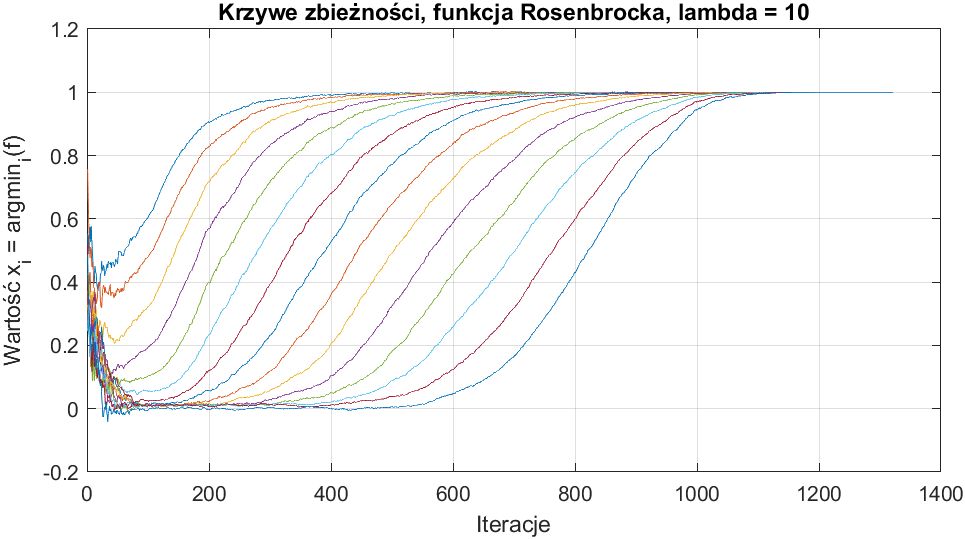
\includegraphics[width=7.5cm]{images/test-lambda-rosenbrock1.png} }}
    \hspace{0.5em}
    \subfloat[\centering $\lambda=60$]{{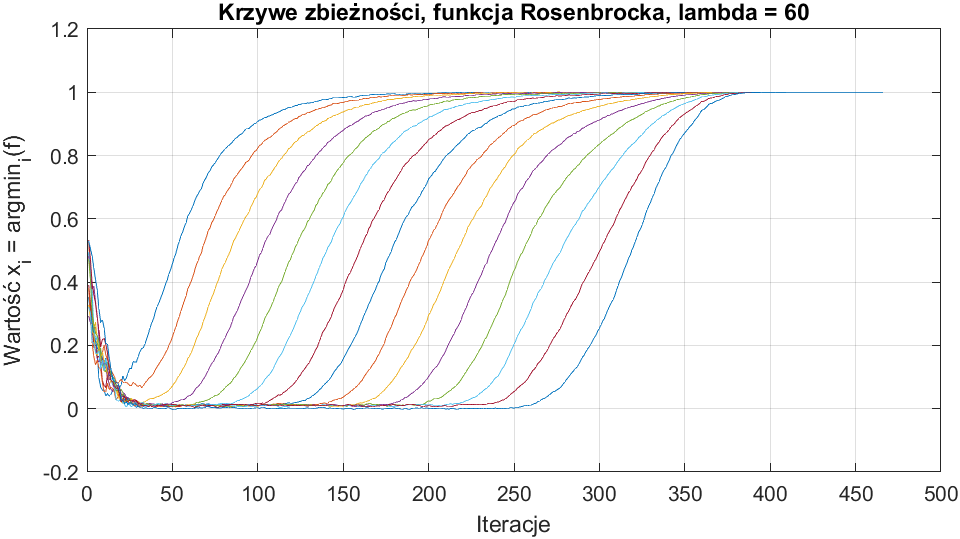
\includegraphics[width=7.5cm]{images/test-lambda-rosenbrock2.png} }}
    \hspace{0.5em}
    \subfloat[\centering $\lambda=110$]{{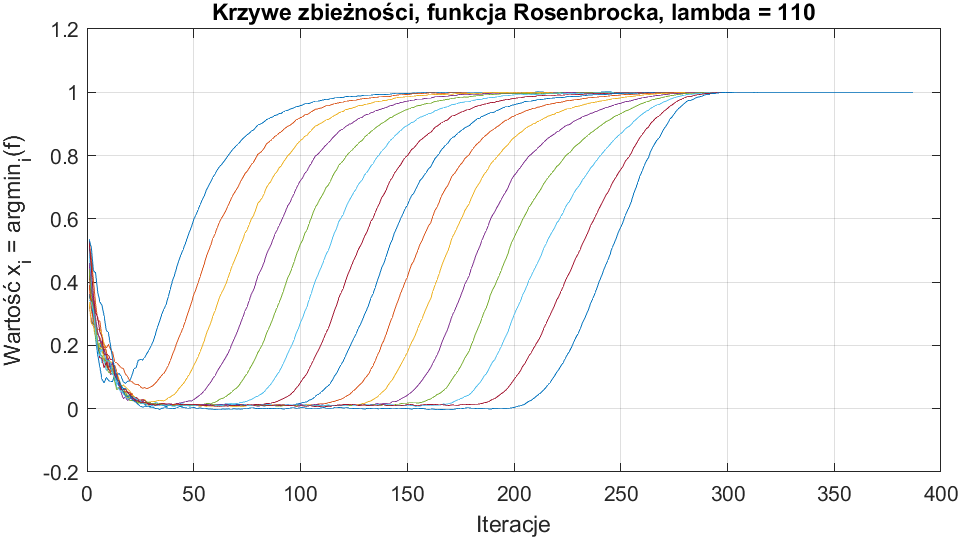
\includegraphics[width=7.5cm]{images/test-lambda-rosenbrock3.png} }}
    \hspace{0.5em}
    \subfloat[\centering $\lambda=160$]{{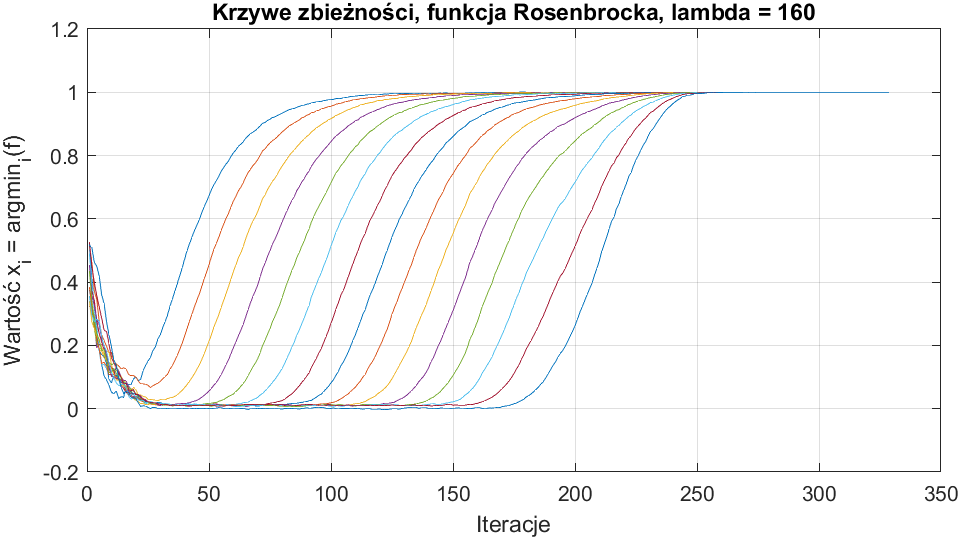
\includegraphics[width=7.5cm]{images/test-lambda-rosenbrock4.png} }}
    \hspace{0.5em}
    \subfloat[\centering $\lambda=210$]{{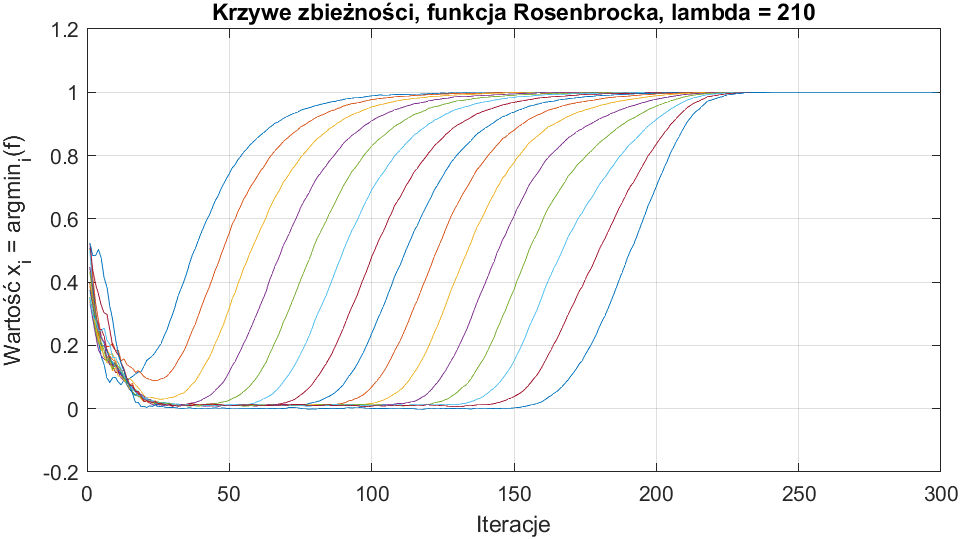
\includegraphics[width=7.5cm]{images/test-lambda-rosenbrock5.png} }}
    \hspace{0.5em}
    \subfloat[\centering $\lambda=260$]{{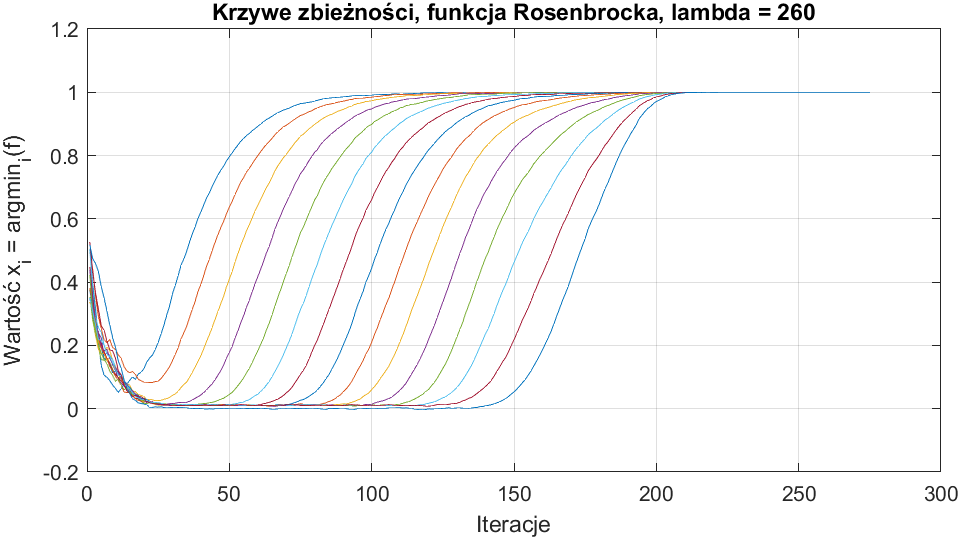
\includegraphics[width=7.5cm]{images/test-lambda-rosenbrock6.png} }}
    \hspace{0.5em}
    \subfloat[\centering $\lambda=310$]{{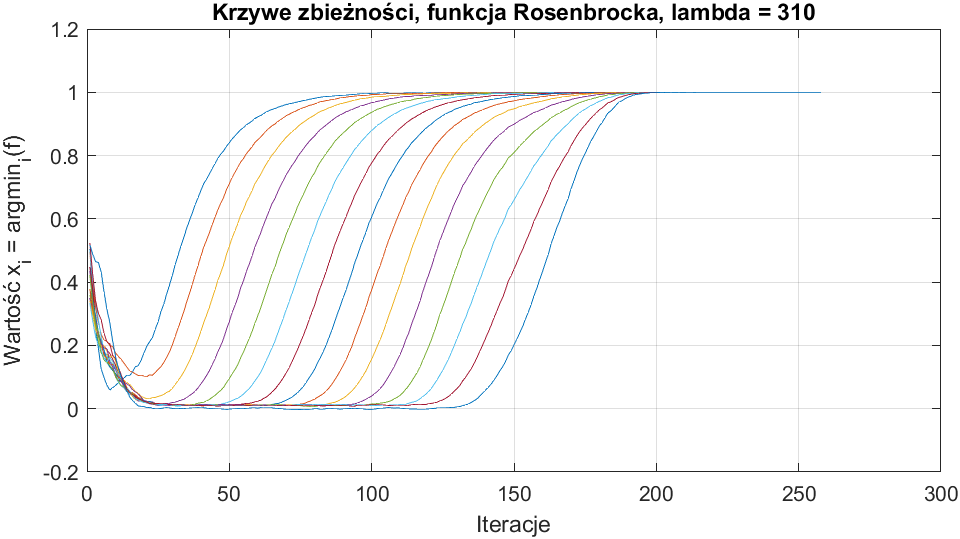
\includegraphics[width=7.5cm]{images/test-lambda-rosenbrock7.png} }}
    \hspace{0.5em}
    \subfloat[\centering $\lambda=360$]{{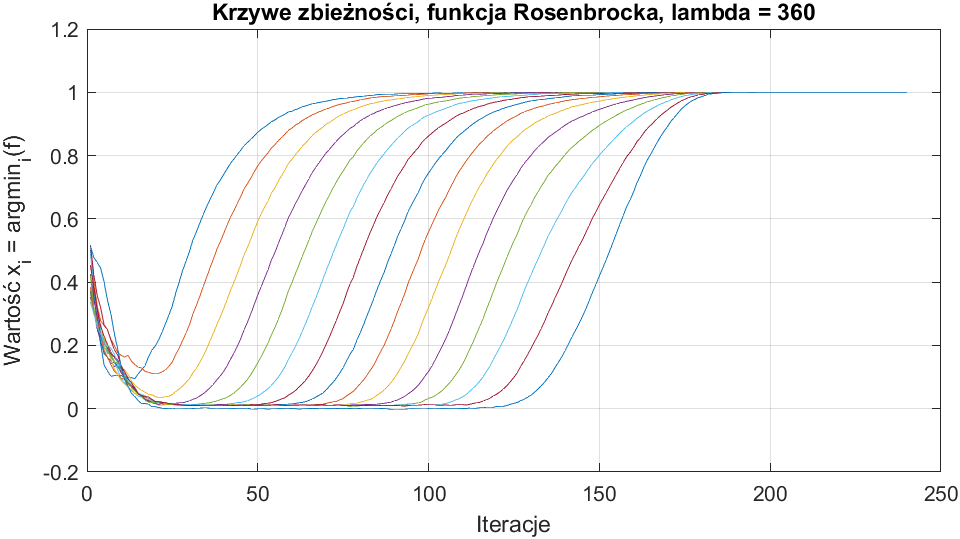
\includegraphics[width=7.5cm]{images/test-lambda-rosenbrock8.png} }}
    \hspace{0.5em}
    \subfloat[\centering $\lambda=410$]{{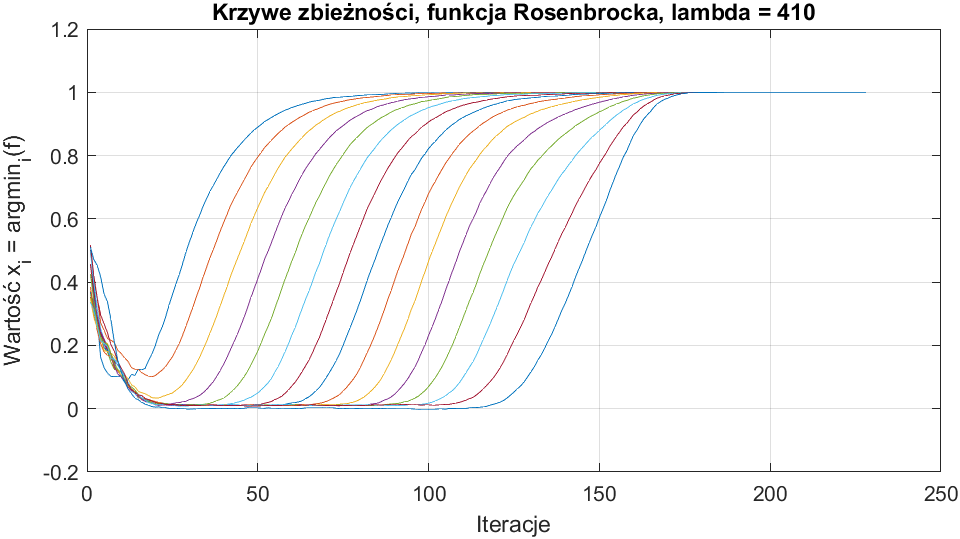
\includegraphics[width=7.5cm]{images/test-lambda-rosenbrock9.png} }}
    \caption{Krzywe zbieżności algorytmu CMA-ES dla funkcji Rosenbrocka przy różnych wielkościach populacji}
    \label{fig:test-lambda-rosenbrock}
\end{figure}

\begin{figure}[H]
	\centering
    \subfloat[\centering $\lambda=10$]{{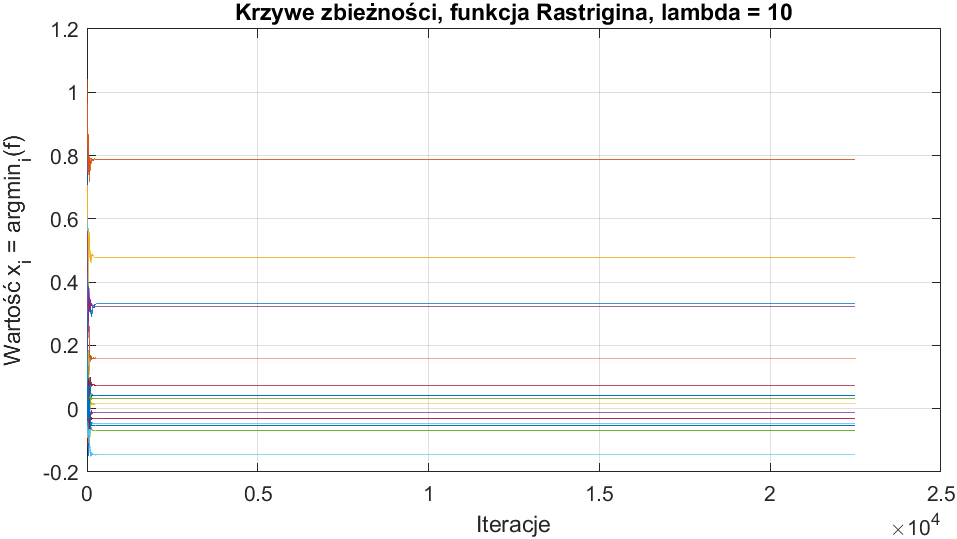
\includegraphics[width=7.5cm]{images/test-lambda-rastrigin1.png} }}
    \hspace{0.5em}
    \subfloat[\centering $\lambda=60$]{{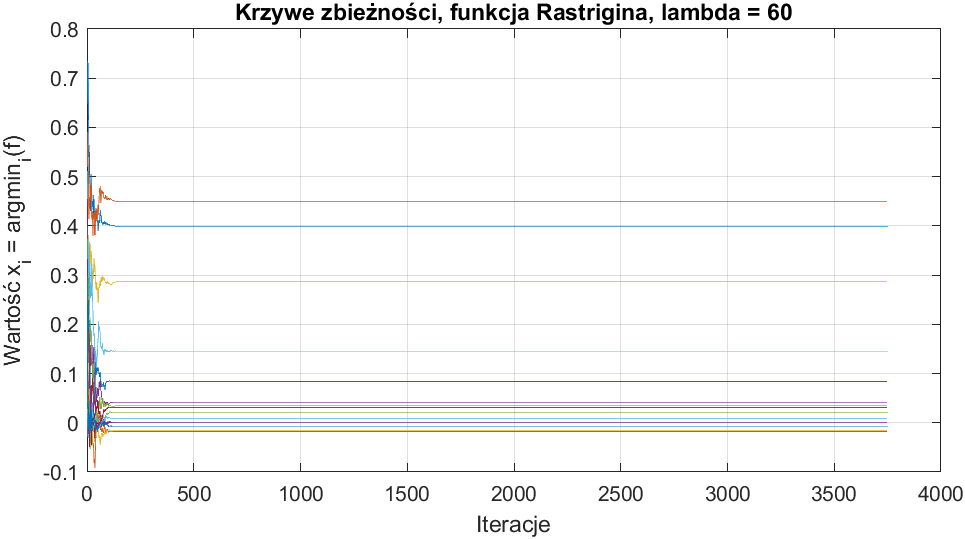
\includegraphics[width=7.5cm]{images/test-lambda-rastrigin2.png} }}
    \hspace{0.5em}
    \subfloat[\centering $\lambda=110$]{{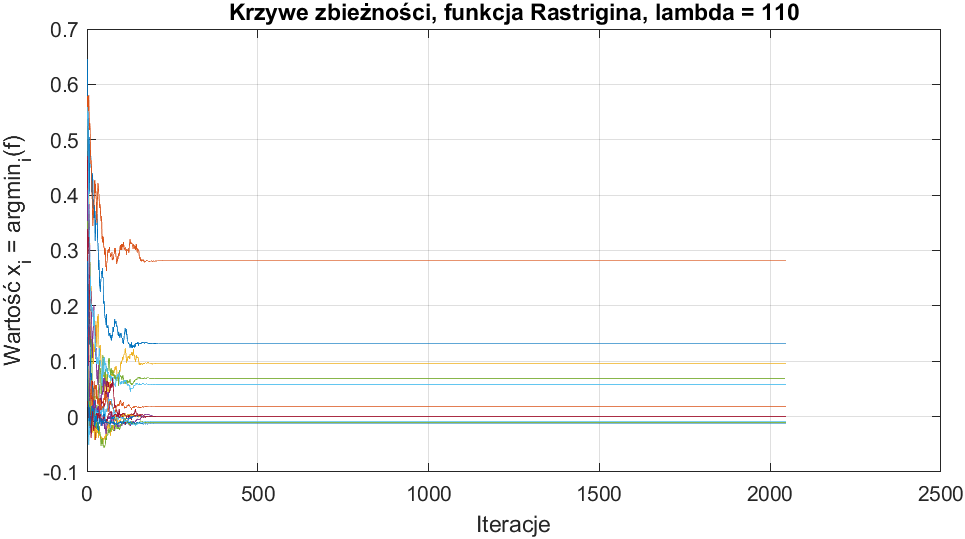
\includegraphics[width=7.5cm]{images/test-lambda-rastrigin3.png} }}
    \hspace{0.5em}
    \subfloat[\centering $\lambda=160$]{{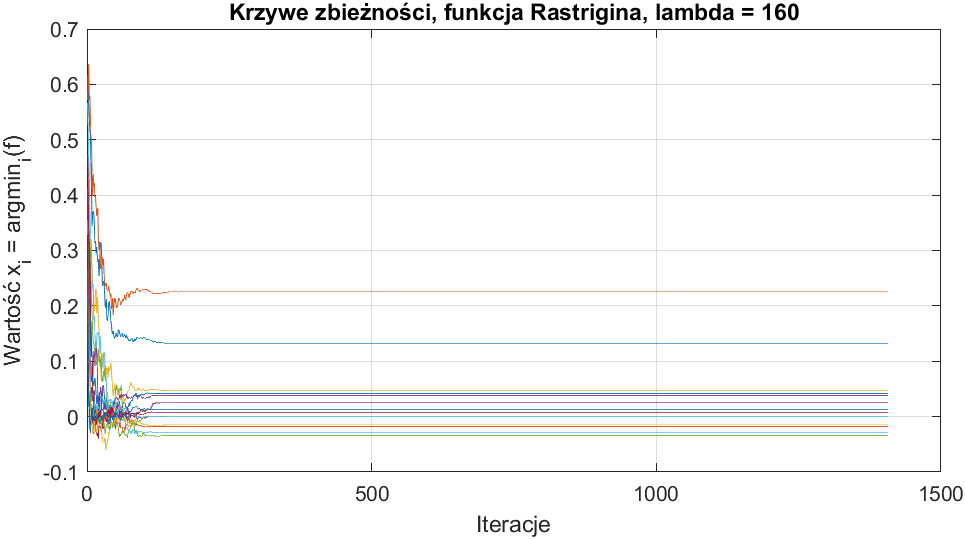
\includegraphics[width=7.5cm]{images/test-lambda-rastrigin4.png} }}
    \hspace{0.5em}
    \subfloat[\centering $\lambda=210$]{{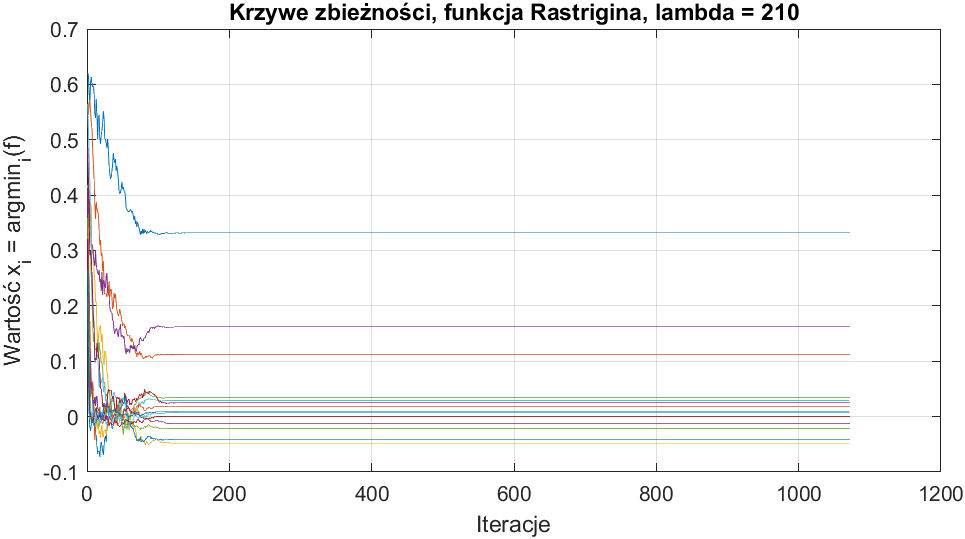
\includegraphics[width=7.5cm]{images/test-lambda-rastrigin5.png} }}
    \hspace{0.5em}
    \subfloat[\centering $\lambda=260$]{{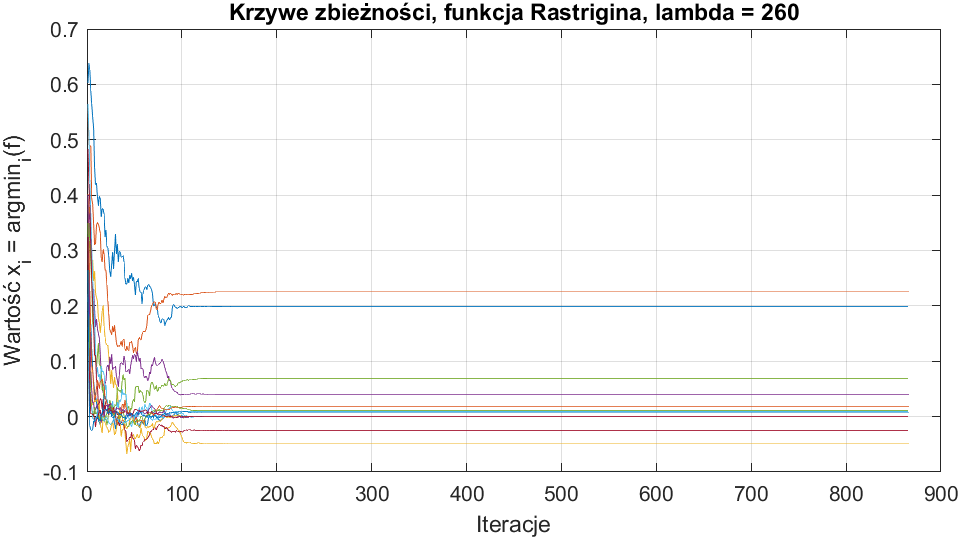
\includegraphics[width=7.5cm]{images/test-lambda-rastrigin6.png} }}
    \hspace{0.5em}
    \subfloat[\centering $\lambda=310$]{{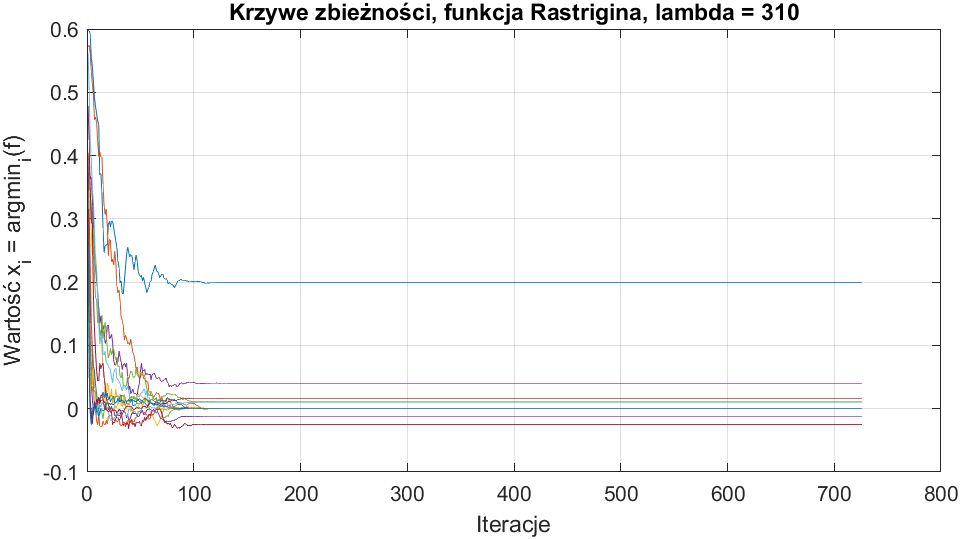
\includegraphics[width=7.5cm]{images/test-lambda-rastrigin7.png} }}
    \hspace{0.5em}
    \subfloat[\centering $\lambda=360$]{{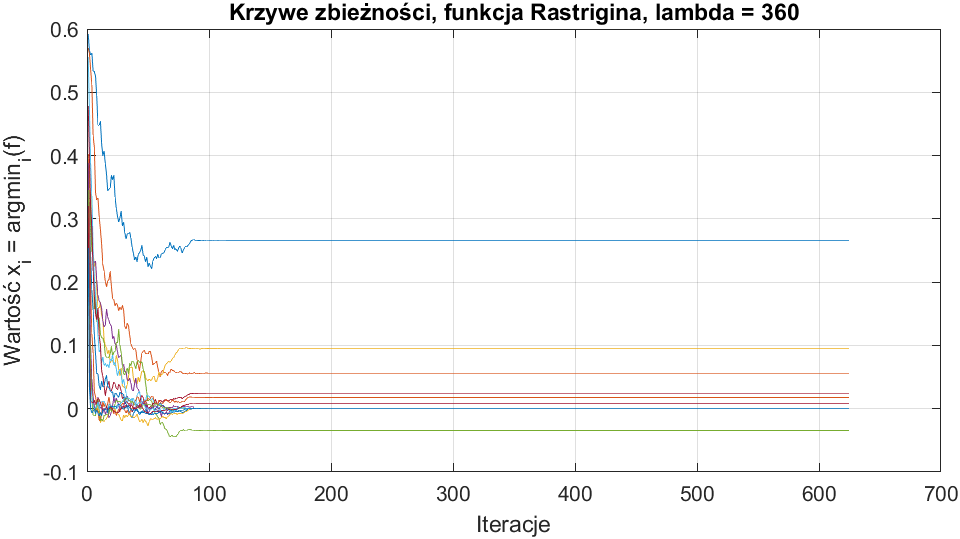
\includegraphics[width=7.5cm]{images/test-lambda-rastrigin8.png} }}
    \hspace{0.5em}
    \subfloat[\centering $\lambda=410$]{{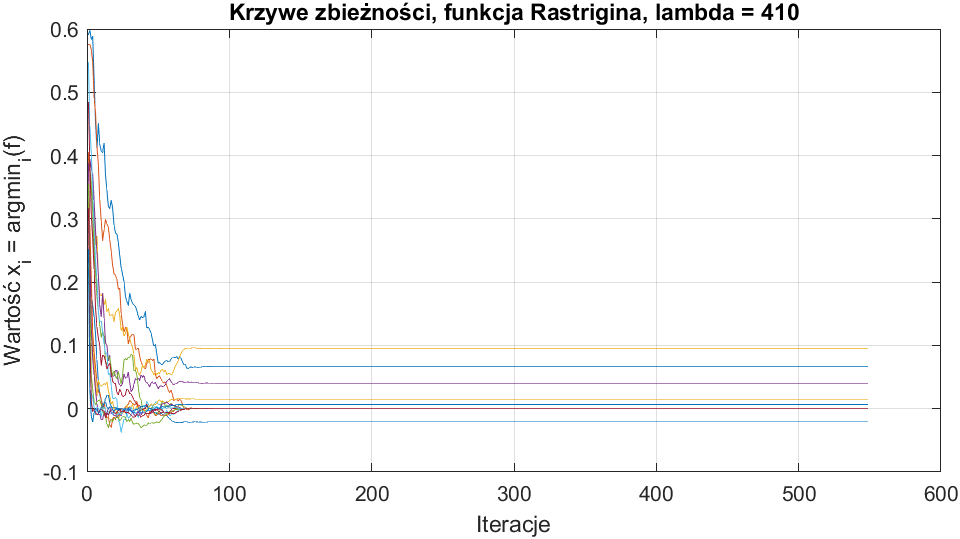
\includegraphics[width=7.5cm]{images/test-lambda-rastrigin9.png} }}
    \caption{Krzywe zbieżności algorytmu CMA-ES dla funkcji Rastrigina przy różnych wielkościach populacji}
    \label{fig:test-lambda-rastrigin}
\end{figure}

Jak widać, pierwsza z funkcji, zbiegała do faktycznego minimum w punkcie o każdej współrzędnej równej 1, dla wszystkich sprawdzanych wartości $\lambda$. Sytuacja prezentuje się jednak zupełnie inaczej dla funkcji Rastrigina. W jej przypadku, globalne minimum (w punkcie o współrzędnych równych 0), nie jest osiągane dla żadnej wartości parametru. Jednak dla trzech ostatnich wartości parametru $\lambda \in \{310, 360, 410\}$, wynik był zdecydowanie bliższy. W celu wybrania najlepszej spośród tych wartości, przeprowadzono również analizę dla algorytmu z wymieraniem oraz analizę dystrybuanty uzyskiwanych rezultatów. Jednak jako, iż nie był to główny temat pracy, podjęto decyzję o pominięciu wykresów w opracowaniu. Niemniej, okazało się, że najlepsze efekty spośród testowanych wartości, były osiągane dla wartości $\lambda = 310$.

Ponownie, zdając sobie sprawę z niedokładności, ale również z drugorzędnego charakteru tego badania, poprzestano na przyjęciu $\lambda = 310$ do dalszych testów.

\subsection{Wybór prawdopodobieństwa i progu wymarcia}
Kolejnymi badanymi parametrami były już parametry dotyczące bezpośrednio mechanizmu wymarcia, czyli prawdopodobieństwo oraz próg wymarcia. Prawdopodobieństwo wymarcia określa szansę z którą dany osobnik populacji zostaje z niej usunięty w procesie wymarcia losowego lub ukierunkowanego. Jednocześnie, w tym drugim przypadku odnosi się to wyłącznie do osobników niespełniających kryterium $k$ najlepszych wyników. Na potrzeby testów, przyjęto sugerowaną w artykule~\cite{ye2021} wartość $k=0.2$, gdyż okazała się ona dawać optymalne wyniki. Próg wymarcia, to z kolei liczba pokoleń przez ile algorytm musi pozostawać w stagnacji, aby uruchomić mechanizm wymarcia.

Zgodnie z intuicją oraz wskazówkami z artykułu~\cite{ye2021}, można przypuszczać wzajemną zależność obu tych parametrów. Z tego powodu, testy zostały przeprowadzone dla różnych kombinacji jednocześnie. Tak też badania zostały przeprowadzone dla $K \in \{10, 20, 30, \dots, 110\}$ oraz $p_{e} \in \{0.1, 0.3, 0.5, 0.7, 0.9\}$. Nie lada zadaniem było dobranie funkcji, dla których różne wartości parametrów powodowały widoczne, nielosowe zmiany. Z tego powodu, po przeanalizowaniu wszystkich funkcji ze zbioru CEC~\cite{CEC}, uznano za najciekawsze rezultaty uzyskane w przypadku analizy funkcji numer 6 ze wspomnianego zbioru (dla wymiarowości równej 10 i 20), jak też 20-wymiarowej funkcji Rastrigina. Ponownie, podobnie jak w przypadku poprzedniej części testów, eksperymenty powtarzano dla 15 różnych ziaren generatora liczb pseudolosowych, uśredniając uzyskane wyniki. Uzyskane wyniki prezentują rysunki \ref{fig:test-extinction-trigger} i \ref{fig:test-extinction-probability}, a także tabele \ref{tab:test-extinction-cec10}, \ref{tab:test-extinction-cec20} oraz \ref{tab:test-extinction-rastrigin}. W przypadku ostatniej funkcji pominięto zaznaczenie na wykresie wartości faktycznego minimum globalnego, gdyż ma ono wartość 0, co zaburzyłoby skalę i czytelność wykresów.

Analizując wyłącznie wyniki uzyskane dla różnych progów wymarcia (uśrednioną dla wszystkich sprawdzanych wartości prawdopodobieństwa wymarcia), warto zwrócić uwagę na nieprzewidywalne zachowanie algorytmów przy niskiej wartości progu. W tych przypadkach algorytm bardzo szybko podejmował decyzję o uruchomieniu mechanizmu wymarcia, co prowadziło do znacznych modyfikacji w dalszym rozwoju populacji. Niestety, ciężko jednoznacznie określić kierunek tych zmian. Dla małego progu wymarcia, dla 10-wymiarowej funkcji ze zbioru CEC~\cite{CEC}, wyniki były gorsze niż podstawowego algorytmu CMA-ES, dla 20-wymiarowej - lepsze, zaś dla funkcji Rastrigina zależało to od typu wymierania. Jednocześnie, wartości progu powyżej 60 praktycznie nie wpływały na zachowanie algorytmu. W tych przypadkach, stagnacja osiągana była już w momencie gdy praktycznie cała populacja grupowała się wokół znalezionego minimum (zazwyczaj lokalnego) i usuwanie części osobników nie zmieniało dynamiki całej grupy.

Z drugiej strony, skupiając się wyłącznie na wartościach prawdopodobieństwa, również ciężko wskazać jednoznaczną tendencję poprawy jakości rozwiązań. Dla funkcji ze zbioru CEC~\cite{CEC}, przy większej wymiarowości, wymieranie poprawiło nieznacznie uzyskany rezultat we wszystkich przypadkach. Dla mniejszej wymiarowości z kolei, uzyskane rezultaty były gorsze. Przy funkcji Rastrigina, ponownie, wszystko zależało to również w dużym stopniu od stosowanego typu wymierania.

Bardziej reprezentatywne w tym przypadku okazało się zestawienie wyników dla obu parametrów, co przedstawiono na wspomnianych już tabelach \ref{tab:test-extinction-cec10}, \ref{tab:test-extinction-cec20} oraz \ref{tab:test-extinction-rastrigin}. Dla czytelności pogrubione zostały w nich najlepsze uzyskane wartości oraz najlepsze średnie. Najlepszą w każdej tabeli dodatkowo podkreślono.

\begin{figure}[H]
	\centering
    \subfloat[\centering 10-wymiarowa funkcja z CEC]{{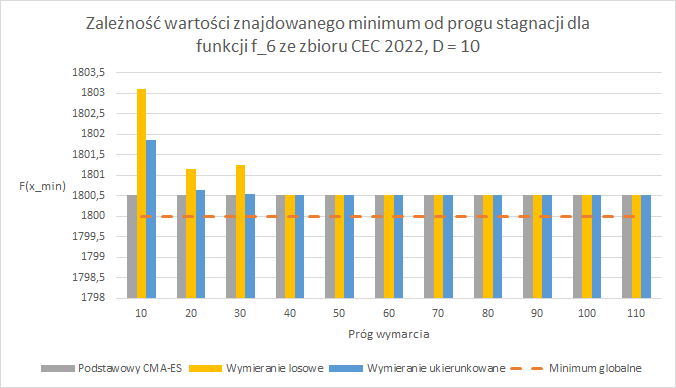
\includegraphics[width=0.75\textwidth]{images/test-extinction-trigger-cec10.png} }}
    \vspace{1em}
    \subfloat[\centering 20-wymiarowa funkcja z CEC]{{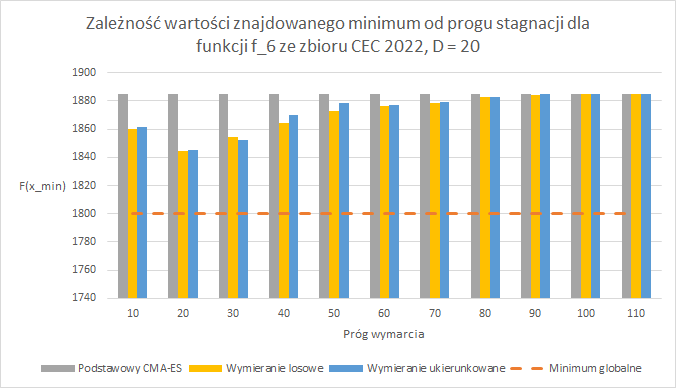
\includegraphics[width=0.75\textwidth]{images/test-extinction-trigger-cec20.png} }}
    \vspace{1em}
    \subfloat[\centering 20-wymiarowa funkcja Rastrigina]{{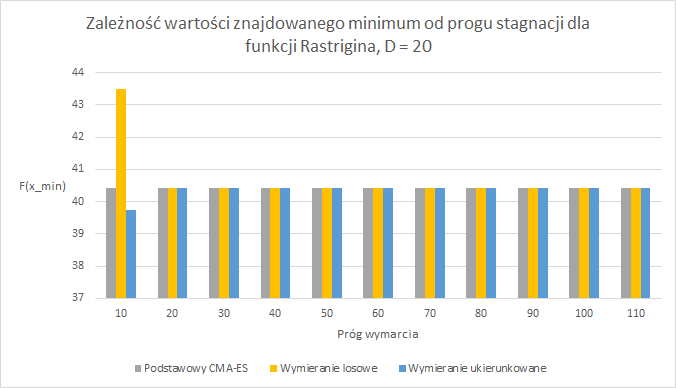
\includegraphics[width=0.75\textwidth]{images/test-extinction-trigger-rastrigin.png} }}
    \caption{Wartości znajdowanego minimum w zależności od algorytmu i progu wymarcia}
    \label{fig:test-extinction-trigger}
\end{figure}

\begin{figure}[H]
	\centering
    \subfloat[\centering 10-wymiarowa funkcja z CEC]{{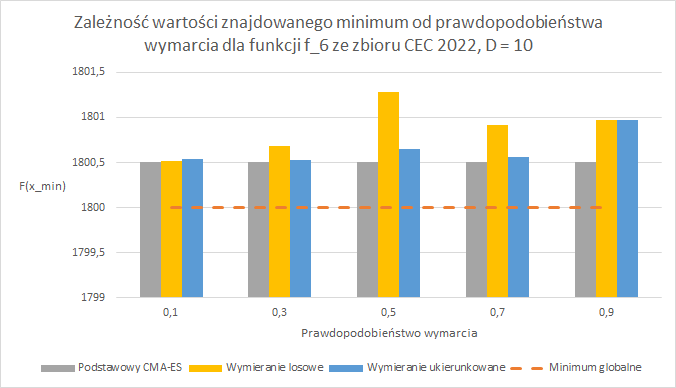
\includegraphics[width=0.75\textwidth]{images/test-extinction-probability-cec10.png} }}
    \vspace{1em}
    \subfloat[\centering 20-wymiarowa funkcja z CEC]{{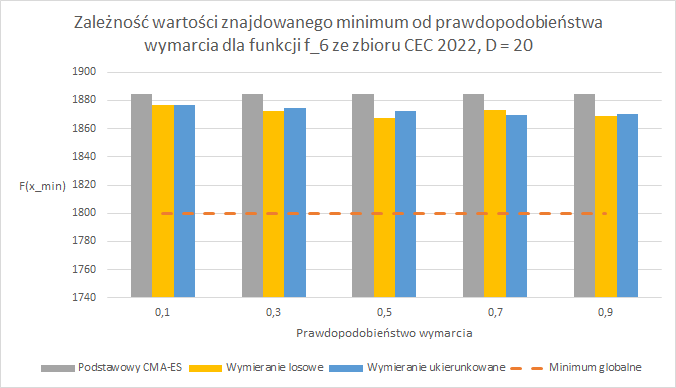
\includegraphics[width=0.75\textwidth]{images/test-extinction-probability-cec20.png} }}
    \vspace{1em}
    \subfloat[\centering 20-wymiarowa funkcja Rastrigina]{{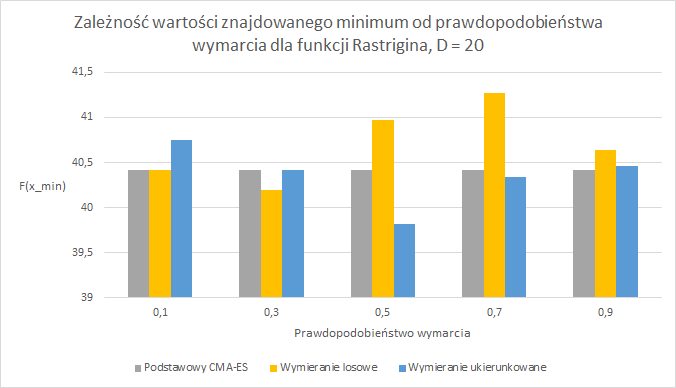
\includegraphics[width=0.75\textwidth]{images/test-extinction-probability-rastrigin.png} }}
    \caption{Wartości znajdowanego minimum w zależności od algorytmu i prawdopodobieństwa wymarcia}
    \label{fig:test-extinction-probability}
\end{figure}

\begin{table}[H]
\caption{Wartość znalezionego minimum w zależności od progu i prawdopodobieństwa wymarcia dla 10 wymiarowej funkcji ze zbioru CEC 2022}
\label{tab:test-extinction-cec10}
\begin{subtable}{\textwidth}
\centering
\begin{tabularx}{0.8\textwidth}{c||X|X|X|X|X||r}
\hline
K & p = 0,1 & p = 0,3 & p = 0,5 & p = 0,7 & p = 0,9 & Średnia  \\ 
\hline \hline
10 & 1800,592 & 1800,604 & 1807,871 & 1803,032 & 1803,383 & 1803,097  \\ 
20 & 1800,538 & 1801,408 & 1800,725 & 1801,551 & 1801,579 & 1801,160  \\ 
30 & 1800,511 & 1801,397 & 1801,388 & 1801,389 & 1801,554 & 1801,248  \\ 
40 & \textbf{1800,507} & \textbf{1800,503} & \textbf{1800,501} & \underline{\textbf{1800,500}} & 1800,558 & 1800,514  \\ 
50 & \textbf{1800,507} & 1800,508 & 1800,510 & 1800,508 & \textbf{1800,507} & \textbf{1800,508}  \\ 
60 & 1800,508 & 1800,508 & 1800,508 & 1800,508 & 1800,508 & \textbf{1800,508}  \\ 
70 & 1800,508 & 1800,509 & 1800,508 & 1800,509 & 1800,509 & \textbf{1800,508}  \\ 
80 & 1800,509 & 1800,509 & 1800,509 & 1800,509 & 1800,509 & 1800,509  \\ 
90 & 1800,509 & 1800,509 & 1800,509 & 1800,509 & 1800,509 & 1800,509  \\ 
100 & 1800,509 & 1800,509 & 1800,509 & 1800,509 & 1800,509 & 1800,509  \\ 
110 & 1800,509 & 1800,509 & 1800,509 & 1800,509 & 1800,509 & 1800,509  \\ 
\hline
Średnia & \textbf{1800,519} & 1800,679 & 1801,277 & 1800,912 & 1800,967 & 1800,871  \\ 
\hline
\end{tabularx}
\caption{Wymieranie losowe}
\end{subtable}

\begin{subtable}{\textwidth}
\centering
\begin{tabularx}{0.8\textwidth}{c||X|X|X|X|X||r}
\hline
K & p = 0,1 & p = 0,3 & p = 0,5 & p = 0,7 & p = 0,9 & Średnia \\
\hline \hline
10 & 1800,616 & 1800,543 & 1801,916 & 1800,942 & 1805,235 & 1801,850 \\
20 & 1800,650 & 1800,603 & 1800,548 & 1800,640 & 1800,814 & 1800,651 \\
30 & 1800,540 & 1800,576 & 1800,536 & 1800,534 & 1800,547 & 1800,547 \\
40 & \textbf{1800,508} & 1800,511 & 1800,532 & 1800,534 & 1800,528 & 1800,522 \\
50 & 1800,509 & \underline{\textbf{1800,508}} & 1800,509 & 1800,509 & 1800,509 & 1800,509 \\
60 & \textbf{1800,508} & 1800,509 & 1800,509 & 1800,509 & \textbf{1800,508} & \textbf{1800,508} \\
70 & 1800,509 & 1800,509 & 1800,509 & 1800,509 & \textbf{1800,508} & 1800,509 \\
80 & 1800,509 & 1800,509 & 1800,509 & 1800,509 & 1800,509 & 1800,509 \\
90 & 1800,509 & 1800,509 & 1800,509 & 1800,509 & 1800,509 & 1800,509 \\
100 & 1800,509 & 1800,509 & 1800,509 & 1800,509 & 1800,509 & 1800,509 \\
110 & 1800,509 & 1800,509 & 1800,509 & 1800,509 & 1800,509 & 1800,509 \\
\hline
Średnia & 1800,534 & \textbf{1800,527} & 1800,645 & 1800,565 & 1800,971 & 1800,648 \\
\hline
\end{tabularx}
\caption{Wymieranie ukierunkowane}
\end{subtable}
\end{table}

\begin{table}[H]
\caption{Wartość znalezionego minimum w zależności od progu i prawdopodobieństwa wymarcia dla 20 wymiarowej funkcji ze zbioru CEC 2022}
\label{tab:test-extinction-cec20}
\begin{subtable}{\textwidth}
\centering
\begin{tabularx}{0.8\textwidth}{c||X|X|X|X|X||r}
\hline
K & p = 0,1 & p = 0,3 & p = 0,5 & p = 0,7 & p = 0,9 & Średnia  \\ 
\hline \hline
10 & 1859,010 & 1854,897 & \textbf{1844,083} & 1878,535 & 1863,387 & 1859,982  \\ 
20 & 1851,389 & \textbf{1842,943} & \underline{\textbf{1833,831}} & \textbf{1847,564} & \textbf{1847,352} & \textbf{1844,616}  \\ 
30 & 1875,891 & 1857,056 & 1851,551 & \textbf{1844,331} & \textbf{1843,214} & 1854,408  \\ 
40 & 1881,413 & 1868,000 & 1861,623 & 1860,547 & 1850,434 & 1864,403  \\ 
50 & 1878,521 & 1876,269 & 1869,386 & 1876,250 & 1865,103 & 1873,106  \\ 
60 & 1878,281 & 1880,609 & 1869,578 & 1878,433 & 1875,149 & 1876,410  \\ 
70 & 1878,684 & 1878,805 & 1874,743 & 1881,048 & 1879,210 & 1878,498  \\ 
80 & 1884,647 & 1884,629 & 1882,457 & 1881,002 & 1881,073 & 1882,762  \\ 
90 & 1884,762 & 1884,822 & 1884,810 & 1884,731 & 1882,383 & 1884,302  \\ 
100 & 1884,744 & 1884,766 & 1884,749 & 1884,819 & 1884,938 & 1884,803  \\ 
110 & 1884,705 & 1884,712 & 1884,717 & 1884,790 & 1884,731 & 1884,731  \\ 
\hline
Średnia & 1876,550 & 1872,501 & \textbf{1867,412} & 1872,913 & 1868,816 & 1871,638  \\ 
\hline
\end{tabularx}
\caption{Wymieranie losowe}
\end{subtable}

\begin{subtable}{\textwidth}
\centering
\begin{tabularx}{0.8\textwidth}{c||X|X|X|X|X||r}
\hline
K & p = 0,1 & p = 0,3 & p = 0,5 & p = 0,7 & p = 0,9 & Średnia \\
\hline \hline
10 & 1859,205 & \textbf{1843,709} & 1867,304 & 1864,366 & 1873,636 & 1861,644 \\
20 & 1857,667 & 1855,907 & \textbf{1836,825} & \underline{\textbf{1827,946}} & 1849,260 & \textbf{1845,521} \\
30 & 1873,642 & 1857,945 & 1856,964 & \textbf{1843,233} & \textbf{1830,299} & 1852,417 \\
40 & 1878,097 & 1881,629 & 1871,690 & 1863,200 & 1857,023 & 1870,328 \\
50 & 1878,087 & 1882,724 & 1875,589 & 1879,141 & 1876,375 & 1878,383 \\
60 & 1880,741 & 1878,555 & 1869,852 & 1878,828 & 1875,892 & 1876,774 \\
70 & 1880,892 & 1884,739 & 1877,575 & 1877,466 & 1875,636 & 1879,262 \\
80 & 1884,575 & 1884,682 & 1884,849 & 1880,835 & 1878,170 & 1882,622 \\
90 & 1884,724 & 1884,730 & 1884,744 & 1884,960 & 1884,910 & 1884,814 \\
100 & 1884,779 & 1884,738 & 1884,876 & 1884,714 & 1884,717 & 1884,765 \\
110 & 1884,729 & 1884,696 & 1884,720 & 1884,708 & 1884,712 & 1884,713 \\
\hline
Średnia & 1877,013 & 1874,914 & 1872,272 & \textbf{1869,945} & 1870,057 & 1872,840 \\
\hline
\end{tabularx}
\caption{Wymieranie ukierunkowane}
\end{subtable}
\end{table}

\begin{table}[H]
\caption{Wartość znalezionego minimum w zależności od progu i prawdopodobieństwa wymarcia dla 20 wymiarowej funkcji Rastrigina}
\label{tab:test-extinction-rastrigin}
\begin{subtable}{\textwidth}
\centering
\begin{tabularx}{0.8\textwidth}{c||X|X|X|X|X||r}
\hline
K & p = 0,1 & p = 0,3 & p = 0,5 & p = 0,7 & p = 0,9 & Średnia  \\ 
\hline \hline
10 & 40,418 & \underline{\textbf{37,984}} & 46,447 & 49,742 & 42,866 & 43,491  \\ 
20 & 40,418 & 40,418 & 40,418 & 40,418 & 40,418 & 40,418  \\ 
30 & 40,418 & 40,418 & 40,418 & 40,418 & 40,418 & 40,418  \\ 
40 & 40,418 & 40,418 & 40,418 & 40,418 & 40,418 & 40,418  \\ 
50 & 40,418 & 40,418 & 40,418 & 40,418 & 40,418 & 40,418  \\ 
60 & 40,418 & 40,418 & 40,418 & 40,418 & 40,418 & 40,418  \\ 
70 & 40,418 & 40,418 & 40,418 & 40,418 & 40,418 & 40,418  \\ 
80 & 40,418 & 40,418 & 40,418 & 40,418 & 40,418 & 40,418  \\ 
90 & 40,418 & 40,418 & 40,418 & 40,418 & 40,418 & 40,418  \\ 
100 & 40,418 & 40,418 & 40,418 & 40,418 & 40,418 & 40,418  \\ 
110 & 40,418 & 40,418 & 40,418 & 40,418 & 40,418 & 40,418  \\ 
\hline
Średnia & 40,418 & \textbf{40,197} & 40,966 & 41,266 & 40,641 & 40,698  \\ 
\hline
\end{tabularx}
\caption{Wymieranie losowe}
\end{subtable}

\begin{subtable}{\textwidth}
\centering
\begin{tabularx}{0.8\textwidth}{c||X|X|X|X|X||r}
\hline
K & p = 0,1 & p = 0,3 & p = 0,5 & p = 0,7 & p = 0,9 & Średnia \\
\hline \hline
10 & 44,013 & 40,431 & \underline{\textbf{33,841}} & \textbf{39,558} & 40,864 & \textbf{39,742} \\
20 & 40,418 & 40,418 & 40,418 & 40,418 & 40,418 & 40,418 \\
30 & 40,418 & 40,418 & 40,418 & 40,418 & 40,418 & 40,418 \\
40 & 40,418 & 40,418 & 40,418 & 40,418 & 40,418 & 40,418 \\
50 & 40,418 & 40,418 & 40,418 & 40,418 & 40,418 & 40,418 \\
60 & 40,418 & 40,418 & 40,418 & 40,418 & 40,418 & 40,418 \\
70 & 40,418 & 40,418 & 40,418 & 40,418 & 40,418 & 40,418 \\
80 & 40,418 & 40,418 & 40,418 & 40,418 & 40,418 & 40,418 \\
90 & 40,418 & 40,418 & 40,418 & 40,418 & 40,418 & 40,418 \\
100 & 40,418 & 40,418 & 40,418 & 40,418 & 40,418 & 40,418 \\
110 & 40,418 & 40,418 & 40,418 & 40,418 & 40,418 & 40,418 \\
\hline
Średnia & 40,745 & 40,419 & \textbf{39,820} & 40,340 & 40,459 & 40,357 \\
\hline
\end{tabularx}
\caption{Wymieranie ukierunkowane}
\end{subtable}
\end{table}

Analizując przedstawione tabele a także mając na uwadze duże wahania skrajnych wartości, uznano za najbardziej reprezentatywne wartości parametrów $p_e = 0,5$ oraz $K = 20$. Prawdopodobieństwo to dawało najczęściej wyniki najlepsze lub od nich nieodległe. Jednocześnie, dla właśnie tej wartości prawdopodobieństwa, najbardziej optymalne rezultaty były osiągane przy progu równym $20$, a żaden z nich nie odbiegał znacznie od najlepszych. 
\section{Analiza wyników na pozostałych funkcjach ze zbioru CEC 2022}
W sekcji tej skupiono się na tych funkcjach dla których odnotowano obiecujące wyniki dla wersji algorytmu z zastosowanym mechanizmem wymarcia.
\subsection{\textit{Shifted and full Rotated Expanded Schaffer's $f6$ function}}
Przesunięta i obrócona, rozszerzona funkcja Schaffera ma wzór:
$$F_3(x) = f_3(M(\frac{0.5(x-o)}{100}) + F_3*, \; F_3* = 600$$
gdzie $M$ to macierz obrotu, $o$ to przesunięcie globalnego minimum, a $f_3(x)$ to rozszerzona funkcja Schaffera, która ma wzór:
$$f_3(x) = g(x_1,x_2)+ g(x_2,x_3) + \dots + g(x_{D-1},x_D) + g(x_D,x_1)$$
$D$ to wymiar zadania, a $g(x,y)$ to funkcja Schaffera o wzorze:
$$g(x,y) = 0.5 + \frac{(\sin^2(\sqrt{x^2 + y^2})-0.5)}{(1+0.001(x^2+y^2))^2}$$
Ze względu na wartość $F_3*$ wartość w minimum globalnym to 600. Wykres funkcji konturowej dla dwóch wymiarów przypomina tafle wody po której roznoszą się okrągłe fale. Funkcja ta posiada wiele minimów lokalnych, oraz jest niesymetryczna.

\begin{figure}[H]
\centering
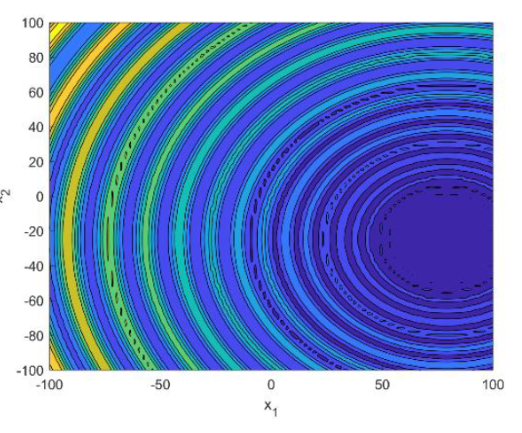
\includegraphics[scale=1]{images/ContourSchaffer.png}
\caption{Konturowy wykres przesuniętej i obróconej, rozszerzonej funkcji Schaffera.}
\end{figure}
\begin{figure}[H]
\centering
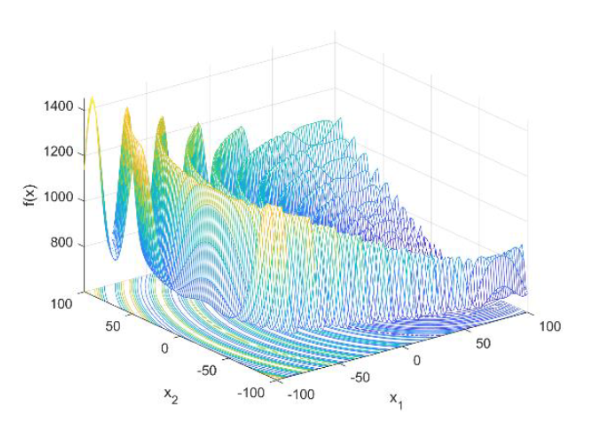
\includegraphics[scale=1]{images/Wykres3DSchaffer.png}
\caption{Wykres 3D przesuniętej i obróconej, rozszerzonej funkcji Schaffera dla 2 wymiarów.}
\end{figure}

Przeprowadzono eksperyment polegający na znalezieniu minimum tej funkcji dla 20 wymiarów, za pomocą podstawowej wersji algorytmu CMA-ES jaki i wersji z wymieraniem ukierunkowanym i losowym. Przyjęto wyznaczoną w poprzednich testach wielkość populacji $310$, próg stagnacji wymagany do wymarcia $20$, prawdopodobieństwo wymarcia $0.5$, a odsetek populacji nie podlegający wymarciu w wersji ukierunkowanej przyjęto $0.2$. Wyniki osiągnięte przez trzy wersje algorytmu, uśrednione dla 15 uruchomień,  zostały przedstawione w tabeli \ref{tab:test-Schaffer}. Widać po nich, że wersja algorytmu CMA-ES z wymieraniem ukierunkowanym osiągnęła średnio lepszy wynik niż podstawowa wersja, gdyż znalazła ona punkt minimum o wartości 666.2754, podczas gdy podstawowa wersja znalazła średnio punkt o wartości 670.3158. Ponadto
odchylenie standardowe dla znalezionego minimum było najmniejsze właśnie dla wymierania ukierunkowanego. Jednakże dla wszystkich wersji, średnia znaleziona wartość była dość odległa od faktycznego minimum.
\begin{table}[H]
\centering
\begin{tabularx}{0.9\textwidth}{c|X|X}
Wersja algorytmu & Znalezione minimum & Odchylenie standardowe\\
\hline
Podstawowy CMA-ES & 670.3158 & 13.4620 \\
\hline
Z wymieraniem ukierunkowanym & \textbf{666.2754} & 8.8949 \\
\hline
Z wymieraniem losowym & 767.4047 & 15.9639\\
\hline 
\hline
Minimum globalne & 600 & -
\end{tabularx}
\caption{Wyniki dla funkcji $f_3$ dla populacji o rozmiarze 310 osobników.}
\label{tab:test-Schaffer}
\end{table}

\subsection{\textit{Shifted and full Rotated Non-Continous Rastrigin's Function}}
Przesunięta i obrócona, nieciągła funkcja Rastrigina ze zbioru CEC 2022 ma wzór:
$$F_4(x) = f_4(M(\frac{5.12(x-o)}{100}) + F_4*, \; F_4* = 800$$
gdzie $M$ to macierz obrotu, $o$ to przesunięcie globalnego minimum, a $f_4(x)$ to funkcja Rastrigina, która ma wzór:
$$f_4(x) = \sum_{i=1}^D(x_u^2 - 10\cos(2\pi x_i) + 10)$$
Ze względu na wartość $F_4*$ wartość w minimum globalnym to 800. Wykres funkcji konturowej dla dwóch wymiarów przypomina ,,wygiętą'' wytłoczkę do jajek. Funkcja ta posiada wiele minimów lokalnych, oraz jest niesymetryczna.\\

\begin{figure}[H]
\centering
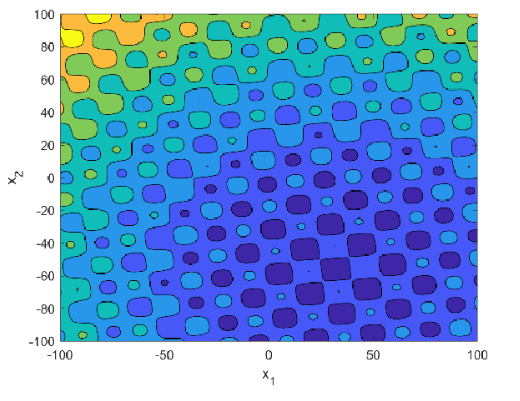
\includegraphics[scale=1]{images/contour-rastrigin.png}
\caption{Konturowy wykres przesuniętej i obróconej, nieciągłej funkcji Rastrigina.}
\end{figure}
\begin{figure}[H]
\centering
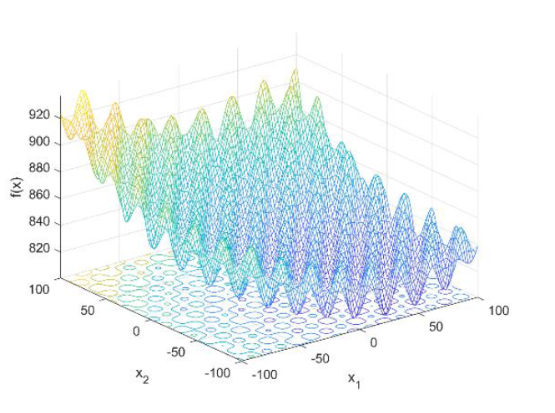
\includegraphics[scale=1]{images/3d-rastrigin.png}
\caption{Wykres 3D przesuniętej i obróconej, nieciągłej funkcji Rastrigina dla 2 wymiarów.}
\end{figure}

Wykonano taki sam eksperyment jak w przypadku funkcji $F_3$. Uśrednione wyniki przedstawiono w tabeli \ref{tab:test-Rastrigin}. Pokazują one, że podobnie jak dla funkcji Schaffera, najlepsze wyniki otrzymano dla wersji z ukierunkowanym wymieraniem. Także odchylenie standardowe było najmniejsze dla tej wersji. Co ciekawe, także losowa wersja osiągnęła lepszy średni wynik niż podstawowa wersja CMA-ES.

\begin{table}[H]
\centering
\begin{tabularx}{0.9\textwidth}{c|X|X}
Wersja algorytmu & Znalezione minimum & Odchylenie standardowe\\
\hline
Podstawowy CMA-ES & 893.3401 & 6.5186 \\
\hline
Z wymieraniem ukierunkowanym & \textbf{887.6355} & 5.4866 \\
\hline
Z wymieraniem losowym &  890.1483 & 6.1983\\
\hline 
\hline
Minimum globalne & 800 & -
\end{tabularx}
\caption{Wyniki dla funkcji $f_4$ dla populacji o rozmiarze 310 osobników.}
\label{tab:test-Rastrigin}
\end{table}

\subsection{ \textit{Shifted and Rotated Levy Function}}
Przesunięta i obrócona Funkcja Levy'ego ze zbioru CEC~\cite{CEC} ma wzór:
$$F_5(x) = f_5(M(\frac{5.12(x-o)}{100}) + F_5*, \; F_5* = 900$$
gdzie $M$ to macierz obrotu, $o$ to przesunięcie globalnego minimum, a $f_5(x)$ to funkcja Levy'ego, która ma wzór:
$$f_5(x) = sin^2(\pi w_1)  + \sum_{i=1}^{D-1}(w_i-1)^2[1+10\sin^2(\pi w_i -1)] + (w_D - 1)^2 [1+sin^2(2\pi w_d)],$$ gdzie $w_i = 1 + \frac{x_i - 1}{4}, \forall i = 1, \dots , D$. Ze względu na wartość $F_5*$ jej minimum ma wartość 900. Funkcja ta podobnie jak $F_4$ i $F_3$ posiada wiele minimum lokalnych.

\begin{figure}[H]
\centering
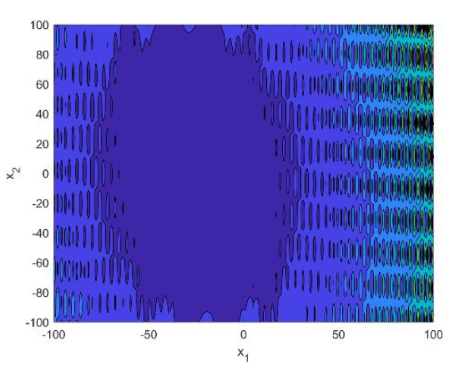
\includegraphics[scale=1]{images/kontur-levy.png}
\caption{Konturowy wykres przesuniętej i obróconej funkcji Levy'ego.}
\end{figure}
\begin{figure}[H]
\centering
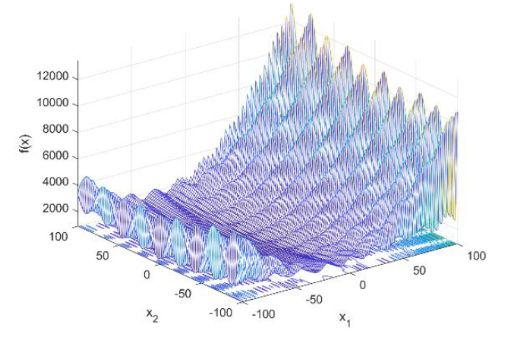
\includegraphics[scale=1]{images/3D-Levy.png}
\caption{Wykres 3D przesuniętej i obróconej funkcji Levy'ego dla 2 wymiarów.}
\end{figure}
Dla funkcje Levy'ego wykonano ten sam eksperyment jak dal funkcji $F_3$ i $F_4$. Wyniki przedstawiono w tabeli \ref{tab:test-Levy}. Widać, że dla tej funkcji algorytm CMA-ES nie jest w stanie znaleźć dobrej wartości. Średnia znaleziona wartość dla podstawowej metody wynosi $3306.6331$, czyli znacznie różni się od faktycznego minimum globalnego, które ma wartość 900. Warto tu zauważyć, że wartości dla wszystkich wersji algorytmu są zbliżone. Pomimo iż dla wymienionych wyżej funkcji $F_3$ i $F_4$, wersja z ukierunkowanym wymieraniem była w stanie znaleźć lepsze rozwiązania, to dla tej funkcji, średnia wartość rozwiązania wyznaczonego za pomocą tej modyfikacji, była gorsza. Ponadto pozwala to zauważyć, że często wartości znajdowane za pomocą wymierania są zbliżone do wartości znalezionych przez podstawowy algorytm CMA-ES i jedynie nieznacznie od nich odbiegają (czasami dając poprawę jak w przypadku $F_3$ i $F_4$, a czasami pogorszenie jak dla funkcji Levy'ego).

\begin{table}[H]
\centering
\begin{tabularx}{0.9\textwidth}{c|X|X}
Wersja algorytmu & Znalezione minimum & Odchylenie standardowe\\
\hline
Podstawowy CMA-ES &  \textbf{3306.6331} & 80.8529 \\
\hline
Z wymieraniem ukierunkowanym & 3308.1225 & 81.2973 \\
\hline
Z wymieraniem losowym &  3309.2155 & 81.2182\\
\hline 
\hline
Minimum globalne & 900 & -
\end{tabularx}
\caption{Wyniki dla funkcji $f_4$ dla populacji o rozmiarze 310 osobników.}
\label{tab:test-Levy}
\end{table}

\section{Podsumowanie}
Niestety, w wyniku przeprowadzonych eksperymentów nie udało się jednoznacznie ustalić, czy modyfikacja algorytmu CMA-ES poprzez wprowadzenie opartego na stagnacji mechanizmu wymarcia wpływa pozytywnie na skuteczność metody. W niektórych przypadkach, dodanie wymarcia pozwala co prawda uzyskiwać wyniki bliższe minimum globalnemu, jednak często przy wymagających funkcjach algorytmy potrafią zostać \textquote{zwiedzione} przez minima lokalne. Podkreśla to moc podstawowej wersji CMA-ES, gdyż pozornie istotna poprawka okazuje się równie często pogarszać działanie wersji podstawowej.

Jednocześnie, osiągniętych rezultatów nie można uznać za nieciekawe. W toku przeprowadzonych eksperymentów, zauważono tendencję wszystkich analizowanych algorytmów do bardzo krótkich okresów stagnacji przed osiągnięciem zbieżności do pewnego minimum lokalnego. Niewątpliwie zmniejszyło to potencjalną skuteczność wymarcia opartego właśnie na stagnacji. Jednocześnie, być może wprowadzenie mechanizmu wymarcia niezależnego od stagnacji, który działałby również na wczesnym etapie przebiegu algorytmu, mogłoby dać ciekawe rezultaty.

Kolejnym dużym problemem była maksymalizacja efektów działania poprzez dobór uniwersalnego progu wymarcia i tolerancji określającej stagnację. W zależności od funkcji, różne wartości parametrów, dla różnych wymiarowości, czy nawet wywołań, były w stanie dawać wyraźnie różne wyniki. Być może, przyjmując konkretną specyfikę przeszukiwanej przestrzeni bądź funkcji celu, dobór tych parametrów byłby łatwiejszy i bardziej efektywny. 

Innym interesującym wnioskiem jest duża zależność jakości działania metody od wielkości wybranej populacji. Wartość tego parametru, mimo iż uznana przez autorów algorytmu za mało istotną, okazała się mieć największy wpływ ze wszystkich sprawdzanych parametrów. 

Poza wielkością populacji, olbrzymi wpływ na wyniki miała również wartość ziarna generatora liczb pseudolosowych. Analizując wywołania dla różnych wartości, wyniki często diametralnie się od siebie różniły. Nasuwa to kolejny bardzo ciekawy potencjalny kierunek dalszych badań. Dla algorytmów o czasie działania ograniczonym z góry przez liczbę wywołań funkcji celu, ciekawym ulepszeniem może okazać się redukowanie liczebności populacji, a następnie dodawanie w ich miejsce innych, zwiększając w ten sposób zdolność do eksploracji, przy stosunkowo stałej wielkości populacji.

\printbibliography
\end{document}